\section{Method}
\label{sec:method}

In this section we propose a new method for automatically selecting good small multiple displays. Our approach takes three inputs from the analyst:
\begin{enumerate}
\item a visualization which the user wants to partition into a small multiple display,
\item a \textit{cognostic}~\cite{Tukey1982,Tukey1985} defined on this visualization type that measures the presence or absence of a visual pattern of interest to the user, and
\item a list of potential partitioning variables.
\end{enumerate}
The output is a scoring of the small multiple displays produced by each partitioning variable.

In the following section, we describe desirable properties for small multiple displays that we use to motivate our approach. The next section describes our method in the context of a running example. We then discuss some straightforward extensions to our basic approach.

\subsection{Goodness-of-Split Criteria}
To guide our approach, we formulated the following four goodness criteria. Partitioning variables should be chosen such that the resulting small multiple displays are:
\begin{itemize}
\item \emph{Visually rich}: We want small multiple displays that convey rich visual patterns, as captured by the cognostic provided by the analyst. In contrast to statistical methods, such as ANOVA, which are based on relatively simple summary metrics with closed-form distributions under some assumptions, most cognostics involve complicated processing and do not follow a known distribution.

\item \emph{Informative}: The purpose of a small multiple display is to help explain patterns in the input visualization. We want to prefer partitioning variables that add information to the display, supporting the user in their analysis. Partitions that randomly split the data are not useful since they don't contain any more information than the original plot.

\item \emph{Well-supported}: For some data sets, particularly those with outliers or with a small number of data points, strong visual patterns can occur by chance. These spurious patterns are misleading; they appear informative, but are not. We would like to detect and downweight such  patterns, guiding analysts to more robust results.

\item \emph{Parsimonious}: A small multiple display with many partitions can be very difficult to read and understand. All things being equal, we want to favor splitting into as few plots as possible, while still providing an informative display.
\end{itemize}

\subsection{Algorithm}

\begin{figure*}
 \centering 
    \begin{subfigure}[t]{1.45in}
        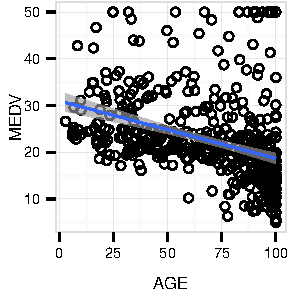
\includegraphics[width=1.45in]{images/AGE-MEDV.pdf}
        \caption{Input plot}
        \label{fig:method_original}
    \end{subfigure}
    \begin{subfigure}[t]{1.5in}
  	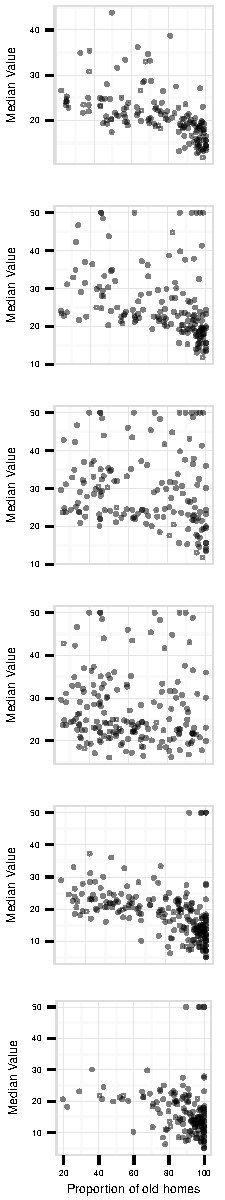
\includegraphics[width=1.5in]{images/TAX.pdf}
	\caption{Partitioned by tax rates}
	 \label{fig:method_actual}
    \end{subfigure}
    \begin{subfigure}[t]{1.5in}
 	 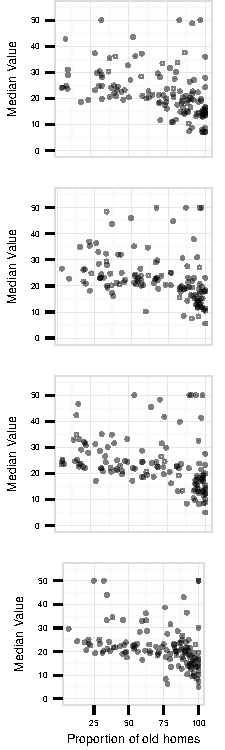
\includegraphics[width=1.5in]{images/randCluster.pdf}
	 \label{fig:method_random}
     \vspace{-0.37cm}
 	\caption{Random partitions}
    \end{subfigure}
     \begin{subfigure}[t]{2.5in}
 	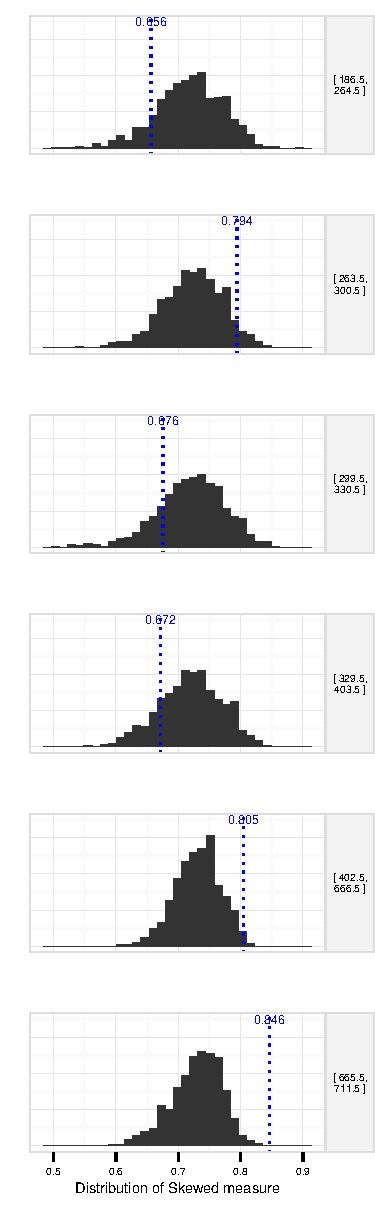
\includegraphics[width=2.5in]{images/hist-TAX.pdf}
	\caption{Distribution of skewness}
	 \label{fig:method_dist}
     \end{subfigure}
   \caption{Illustration of our method of evaluating small multiple displays. (a) Input bivariate relationship of interest. (b) Partitions determined by the levels of XX. (c) Randomly permuted partitions of data. (d) Distribution of X measures for randomly permuted partitions. The overlaid blue lines are the corresponding true scores of the partitions determined by XX in (b).}
\end{figure*}

Our approach is based on a simple intuition: effective small multiple displays are those whose component plots have cognostic scores that are very unlikely to have arisen due to chance. In this section, we describe a method for evaluating this likelihood using a \emph{randomized permutation test}, which is a non-parametric statistical significance test. In the following section, we demonstrate that this approach produces results that conform to our given goodness criteria.

Our algorithm works as follows: for a given partitioning variable, we evaluate the cognostic score on each component plot of the resulting small multiple, resulting in a vector of \emph{true} scores. We then repeatedly randomly permute the values of the partitioning variable, assigning each data point to a random partition, and reevaluate the cognostic score for each component plot. These randomized cognostic scores give us a vector of ``null distributions'', reflecting how likely different cognostic scores are to arise just by chance for each plot.

We then compare the true scores to the ``null distributions'' by evaluating a z-score. This gives us a normalized measure that indicates how far the true cognostic is from that of a random partition. The z-score for each component plot $p_i$ is as follows:
$$z_i = \frac{(X_i-\mu_i)}{\sigma_i}$$ 
where $X_i$ is the true score of the $i$-th partition of the $k$ partitions and $\mu_i$ and $\sigma_i$ are the mean and standard deviation of the cognostic measures over the $r$ random permutations for the $i$-th partition.

Finally, to get a score for the whole small multiple display, we use the maximum absolute z-score across all the plots: 
$$z = \max_{i=1}^k |z_i|$$ 
Combining scores with the sum aggregation would not penalize high-cardinality variables that result in many partitions. Similarly, the mean aggregation would reduce the effect outlier scores while we want to discover such component plots. (NEED cleaning here)

To demonstrate this algorithm, consider the example in Figure~\ref{fig:method_original} showing the relationship between the median value of owner-occupied homes in $\$1000s$ and the proportion of owner-occupied units built prior to 1940. This dataset contains information collected by the U.S Census Service concerning housing in the area of Boston, Massachusetts~\cite{Harrison1978}. We see that as the age of houses increases, their median value decreases and there are more older houses in the Boston area

The analyst might wonder whether any of the other variables in the dataset could partition the view, isolating and explaining the skewness. So, to discover splits that are unusually skewed, the analyst selects the Skewed scagnostic~\cite{Wilkinson2005} as the non-parametric cognostic estimating the density of points in a scatterplot. 

Figure~\ref{fig:method_actual} shows the small multiple display resulting from partitioning on the binned measure of the property-tax rate per $\$10,000$. We compute it for each of the six component plots to form the vector of true scores. In the six partitions of equal count~\cite{Becker1996}, we see five that share the skewed pattern in the original view with a larger proportion of houses close to $100$ years old. However, for houses with property tax values in the range of 300--430 we see a dispersed pattern with a lot more houses that are 50--60 years old. Therefore, this variable reveals an informative partitioning of the original view as it diverges from the original.

We randomly permute the assignment of data points to the six partitions to produce a partitioning as in Figure~\ref{fig:method_random} where all the partitions look similar to the original bivariate relationship. We compute cognostic scores for each component plot. Then, we repeat this random permutated assignment and score computation to produce a distribution of cognostic scores for each component plot as seen in the Figure~\ref{fig:method_dist}. The true scores of the partitioning by the tax rate are overlaid as blue lines to establish a sense of the distance from random partitionings. We apply the non-parametric significance test to determine how significant the difference is and take the maximum of the z-scores from the partitions which ranks the tax rate variable at the top with a score of $4.144$.

\subsection{Extensions}
One advantage to our approach is that it can easily be extended in a number of different ways. For example, our method naturally works on discrete partitioning variables. For continuous variables, discrete partitions can be created through various disjoint binning techniques~\cite{Freedman1981,Scott2009}. Alternatively, overlapping bins (shingles) could also be used~\cite{Becker1996}. In either case, our approach can be extended to handle binning by first permuting the continuous variable and then applying the binning algorithm to partition the data.

While we frame our algorithm in terms of scoring single variables, it is trivial to combine two discrete variables into a new discrete variable by crossing or nesting the levels of each variables~\cite{Wilkinson2005GG,Stolte2002}. Doing so would allow our algorithm to consider combinations of variables. However, unlike powerful statistical variable selection techniques, such as lasso regression, this approach is relatively ad hoc.

Finally, we have described our algorithm in terms of a permutation test, which ignores sampling error in the data set. This is correct in many common analytic scenarios where the entire population is in the data set. If, however, the user wanted to account for sampling error when scoring small multiple displays, they could instead use bootstrapping to build the null distribution. The structure of the approach would be unchanged.

